%   Borrowed from A. Shafiei
%
%   Copyright (c)  2023  A. Shafiei
%   Permission is granted to copy, distribute and/or modify this document
%    under the terms of the GNU Free Documentation License, Version 1.3
%    or any later version published by the Free Software Foundation;
%    with no Invariant Sections, no Front-Cover Texts, and no Back-Cover Texts.
%    A copy of the license is included in the section entitled "GNU
%    Free Documentation License".

\documentclass[
    aspectratio=169,
    dvipsnames,
    svgnames,
    x11names
]{beamer}

% URLs and hyperlinks ---------------------------------------
\usepackage{hyperref}
\hypersetup{
    colorlinks=true,
    linkcolor=NavyBlue,
    filecolor=magenta,      
    urlcolor=blue,
}
\usepackage{xurl}
%---------------------------------------------------

\usefonttheme{serif}
\usepackage{listings}
\usepackage{docs/style}

\newcommand{\token}[1]{\left\langle\text{\lr{\textbf{id}}}, \text{\lr{#1}}\right\rangle}

\usepackage{xepersian}
\settextfont{Yas}

% Persian specific
\newcommand{\itmsep}[1]{\raggedleft\setlength\itemsep{#1}}
\newcommand{\itemr}{\raggedleft\setlength\itemsep{3mm}}
\newcommand{\fn}[2]{{\LR{\footnote[frame,#1]{{~\LR{#2}}}}}}
\newcommand{\fnn}[1]{{\LR{\footnote[frame]{{~\LR{#1}}}}}}
\newcommand{\m}[1]{\ensuremath{\mathnormal{#1}}}
\newcommand{\mc}[1]{\ensuremath{\mathtt{#1}}}
\newcommand{\scl}{\ensuremath{\Sigma^*}\xspace}
\newcommand{\gcl}{\ensuremath{\Gamma^*}\xspace}
\newcommand{\gin}{\ensuremath{\mathnormal{\in}}\xspace}
%\newcommand{\gand}{\ensuremath{\mathnormal{\land}}\xspace}
\newcommand{\gand}{\&\&\xspace}
\newcommand{\alglr}{\LTR\ttfamily\small}
\newcommand{\st}[1]{\ensuremath{\mathnormal{\{#1\}}}\xspace}
\newcommand{\gst}[1]{\ensuremath{\mathnormal{\{\text{\texttt{#1}}\}}}\xspace}
\newcommand{\cpp}{C++\xspace}
\newcommand{\enc}[1]{\ensuremath{\mathnormal{\langle#1\rangle}}\xspace}
\newcommand{\abo}[1]{\ensuremath{\mathnormal{O(#1)}}\xspace}
\newcommand{\aso}[1]{\ensuremath{\mathnormal{o(#1)}}\xspace}
\newcommand{\aom}[1]{\ensuremath{\mathnormal{\Omega(#1)}}\xspace}
\newcommand{\ath}[1]{\ensuremath{\mathnormal{\Theta(#1)}}\xspace}
\newcommand{\dom}[2]{\ensuremath{\mathnormal{\Big[ \dfrac{#1}{#2} \Big]}}\xspace}

\newcommand{\Proc}[2]{\Statex \textbf{procedure} \textsc{#1}(#2)}
\newcommand{\Func}[2]{\Statex \textbf{function} \textsc{#1}(#2)}
\newcommand{\To}{\textbf{to}\xspace}

\newcommand\pro{\ensuremath{\rightarrow}\xspace}
\newcommand\der{\ensuremath{\Rightarrow}\xspace}
\newcommand\ders{\ensuremath{\stackrel{\mbox{*}}{\Rightarrow}}\xspace}
\newcommand{\dern}[1]{\ensuremath{\stackrel{\mbox{\small #1}}{\Rightarrow}}\xspace}
\newcommand\move{\ensuremath{\vdash}\xspace}
\newcommand\moves{\ensuremath{\stackrel{\small *}{\vdash}}\xspace}
\newcommand{\movesn}[1]{\ensuremath{\stackrel{\small *}{\vdash_{#1}}}\xspace}
\newcommand{\moven}[1]{\ensuremath{\mathnormal{\vdash_{#1}}}\xspace}

\newcommand{\code}[1]{{\LR{\texttt{#1}}}}
\newcommand{\txtlr}[1]{\text{\LR{#1}}}


% Abbreviations
\newcommand{\ie}{\latin{i.e.,~}}
\newcommand{\eg}{\latin{e.g.,~}}
\newcommand{\cf}{\latin{cf.~}}
\newcommand{\etal}{\latin{et al.~}}
\newcommand{\etc}{\unskip~\latin{etc.}\xspace}
\newcommand{\apriori}{\latin{a priori}}
\newcommand{\wrt}{\latin{w.r.t.~}}
%\newtheorem{theorem}{Theorem}

\newcommand\NN{\ensuremath{\mathbb{N}}\xspace}
\newcommand\RR{\ensuremath{\mathbb{R}}\xspace}
\newcommand\NNS{\ensuremath{\mathbb{N}^*}\xspace}
\newcommand\NNZ{\ensuremath{\mathbb{N}\backslash\{0\}}\xspace}
\newcommand\RRP{\ensuremath{\mathbb{R}^+}\xspace}
\newcommand\vect[1]{\ensuremath{\boldsymbol{\vec{#1}}}}
\newcommand\MP{\ensuremath{\mathcal{P}}\xspace}

\newcommand\de{\mathrel{\bullet\mkern-2.5mu{\rightarrow}}}
\newcommand\ue{\mathrel{\bullet\mkern-3mu{-}\mkern-3mu\bullet}}

\DeclareMathOperator*{\argmax}{arg\,max}
\DeclareMathOperator*{\argmin}{arg\,min}

\DeclareMathOperator{\lcm}{lcm}
\DeclareMathOperator{\Spec}{Spec}
\DeclareMathOperator{\Res}{Res}
%\DeclareMathOperator{\land}{and}

\newcommand{\fl}[1]{\ensuremath{\lfloor #1 \rfloor}}
\newcommand{\bfl}[1]{\ensuremath{\big\lfloor #1 \big\rfloor}}
\newcommand{\Bfl}[1]{\ensuremath{\Big\lfloor #1 \Big\rfloor}}
\newcommand{\bgfl}[1]{\ensuremath{\bigg\lfloor #1 \bigg\rfloor}}
\newcommand{\Bgfl}[1]{\ensuremath{\Bigg\lfloor #1 \Bigg\rfloor}}

\newcommand{\cl}[1]{\ensuremath{\lceil #1 \rceil}}
\newcommand{\bcl}[1]{\ensuremath{\big\lceil #1 \big\rceil}}
\newcommand{\Bcl}[1]{\ensuremath{\Big\lceil #1 \Big\rceil}}
\newcommand{\bgcl}[1]{\ensuremath{\bigg\lceil #1 \bigg\rceil}}
\newcommand{\Bgcl}[1]{\ensuremath{\Bigg\lceil #1 \Bigg\rceil}}

\newcommand{\mtx}[1]{\begin{pmatrix} #1 \end{pmatrix}}
\newcommand{\smtx}[1]{\begin{psmallmatrix} #1 \end{psmallmatrix}}

\definecolor{commentgreen}{RGB}{2,112,10}
\definecolor{eminence}{RGB}{108,48,130}
\definecolor{brightmaroon}{rgb}{0.76, 0.13, 0.28}
\definecolor{darkred}{rgb}{0.55, 0.0, 0.0}
\lstset {
    language=C++,
    frame=tb,
    tabsize=4,
    showstringspaces=false,
    numbers=left,
    %upquote=true,
    commentstyle=\color{commentgreen},
    keywordstyle=\color{eminence},
    stringstyle=\color{darkred},
    basicstyle=\small\ttfamily, % basic font setting
    emph={int,char,double,float,unsigned,long,short,void,bool},
    emphstyle={\color{blue}},
    %escapechar=\&,
    % keyword highlighting
    %classoffset=1, % starting new class
    %otherkeywords={>,<,.,;,-,!,=,~},
    %morekeywords={>,<,.,;,-,!,=,~},
    %keywordstyle=\color{weborange},
    %classoffset=0,
}

\makeatletter
\NewDocumentCommand{\LeftComment}{s m}{%
	\IfBooleanF{#1}{\hspace*{\ALG@thistlm}}\textcolor{commentgreen}{\(~\triangleright\) #2}}
\makeatother


\title{\lr{Compiler Design}}
\author{مهدی حق‌وردی}

\institute{
\\
\includegraphics[height=1.2cm]{logos/logo}\\
دانشگاه‌ اصفهان
}
\date{}

\DeclareRobustCommand\cs[1]{\texttt{\char`\\#1}}
\begin{document}

\begin{frame}[plain]
\begin{center}
به نام خدا
\end{center}
\maketitle
\end{frame}

\setcounter{framenumber}{0}
\raggedleft

\begin{frame}{فهرست مطالب}
\begin{flushright}
\tableofcontents
\end{flushright}
\end{frame}

\section{مقدمه}
\begin{frame}{مقدمه}
\begin{itemize}\itemr
\item[-]
در این ارائه به بررسی معماری کامپیوتر می‌پردازیم
\item[-]
ابتدا سرگذشت و روند تکاملی معماری را بررسی می‌کنیم،
\item[-]
سپس به معرفی اجزای اصلی یک کامپیوتر می‌پردازیم،
\item[-]
پس از آن به داخل \lr{CPU} می‌رویم و معماری‌های متفاوت آن را می‌بینیم،
\item[-]
سپس در مورد آینده‌ی معماری کامپیوتر صحبت می‌کنیم
\item[-]
و در آخر، تاثیر هوش مصنوعی به روی معماری کامپیوتر را بررسی می‌کنیم.
\end{itemize}
\end{frame}
\section{معرفی}
\begin{frame}{معرفی}
\begin{itemize}\itemr
\item[-]
زبان‌های برنامه‌نویسی، نمادها و ابزاری برای توصیف محاسبات برای انسان‌ها و کامپیوتر‌ها هستند.
\item[-]
جهانی که ما می‌شناسیم به زبان‌های برنامه‌نویسی وابستگی بسیار زیادی دارد، چون تمام نرم‌افزارهای روی کامپیوتر‌ها دنیا با زبانی نوشته شده‌اند.

\item[-]
اما قبل از اینکه بتوانیم آنها را \textbf{اجرا (\lr{run})} کنیم، باید بتوانیم آنها را به حالتی تبدیل کنیم که پردازنده‌های ما بتوانند آ‌ن‌ها را اجرا کنند.
\end{itemize}
\end{frame}

\section{پردازشگر‌های زبان}
\begin{frame}[fragile]{پردازش‌گر‌های زبان}
\begin{itemize}\itemr
\item[-]
به بیان ساده، کامپایلر برنامه‌ایست که می‌تواند یک برنامه را با یک زبان (\lr{\textit{source} language}) بخواند، و معادل آن را به زبانی دیگر ترجمه کند  (\lr{\textit{targer} language}.)
\vspace{5mm}
\begin{figure}[H]
\begin{center}
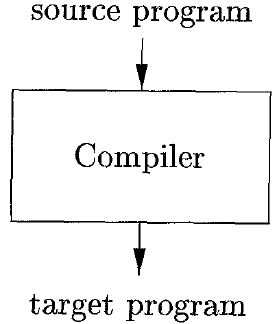
\includegraphics[width=0.3\textwidth, height=0.6\textheight, angle=1]{docs/images/sct}
\end{center}
\end{figure}
\end{itemize}
\end{frame}

\begin{frame}{برنامه‌ی ترجمه شده}
\begin{itemize}\itemr
\item[-]
اگر برنامه‌ی تولید شده، یک 
\lr{executable machine-language program}
باشد، می‌توان آن را مستقیما توسط پردازنده اجرا کرد.
\vspace{5mm}
\begin{figure}[H]
\begin{center}
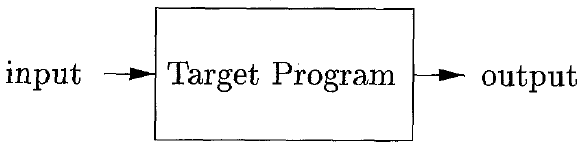
\includegraphics[width=0.6\textwidth, height=0.3\textheight, angle=0.5]{docs/images/executable}
\end{center}
\end{figure}
\end{itemize}
\end{frame}

\begin{frame}{مفسر}
\begin{itemize}\itemr
\item[-]
نوع دیگری از پردازش‌گر‌های زبانی، مفسرها هستند که بجای تبدیل زبان به زبان دیگر (\lr{\textit{target}})، خود مستقیما مسئول اجرای زبان اول (\lr{\textit{source}}) می‌شوند.
\vspace{5mm}
\begin{figure}[H]
\begin{center}
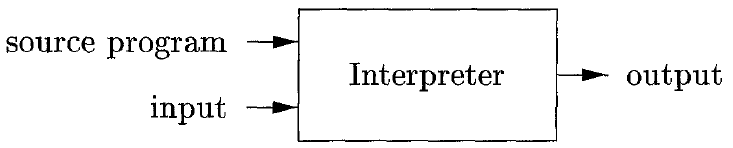
\includegraphics[width=0.7\textwidth, height=0.3\textheight, angle=0]{docs/images/interpreter}
\end{center}
\end{figure}
\end{itemize}
\end{frame}

\begin{frame}{یک سیستم پردازشگر زبان - \lr{Preprocessor}}
\begin{figure}[H]
\begin{center}
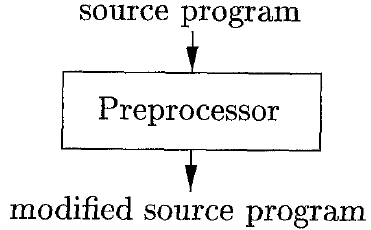
\includegraphics[width=0.5\textwidth, height=0.5\textheight, angle=0.6]{docs/images/preprocessor}
\end{center}
\end{figure}
\end{frame}

\begin{frame}[fragile]{\lr{Preprocessor}}
\begin{itemize}\itemr
\item[-]
زبان‌های کهنی مثل \lr{C} و \lr{C++} سیستم \lr{moduling} و ساختاربندی منظمی برای جدا کردن \lr{source code}هایشان نداشتند.

\item[-]
اما زبان‌های جدیدتر مثل \lr{Python} چنین سیستمی را دارند.

\begin{latin}
\begin{lstlisting}[language=python]
import math
from csv import reader, writer
\end{lstlisting}
\end{latin}
\end{itemize}
\end{frame}

\begin{frame}{\lr{Preprocessor}}
\begin{itemize}\itemr
\item[-]
به همین دلیل، آنها نیاز داشتند که وقتی برنامه‌ای که نوشته‌اند را به چندین فایل تقسیم کرده‌اند، کامپایل کنند، برنامه‌ای تمام \lr{source code}هایشان را به یک 
\lr{source code}
واحد تبدیل کرده و آن را به کامپایلر بدهند.

\item[-]
که بخاطر این نیاز، نرم‌افزاری به نام 
\lr{Preprocessor}
نوشته شد.
\end{itemize}
\end{frame}

\begin{frame}{\lr{Preprocessor}}
\begin{figure}[H]
\begin{center}
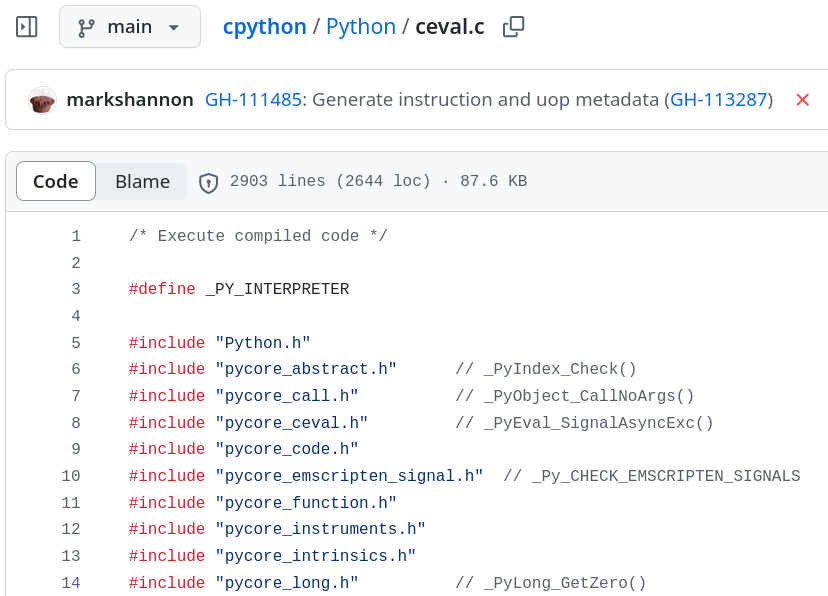
\includegraphics[width=0.6\textwidth, height=0.7\textheight]{docs/images/include}
\end{center}
\end{figure}
\end{frame}

\begin{frame}{\lr{Preprocessor}}
\begin{itemize}\itemr
\item[-]
با \lr{Preprocessor}ها می‌توان ماکرو به زبان اضافه کرد.

\vspace{5mm}
\begin{figure}[H]
\begin{center}
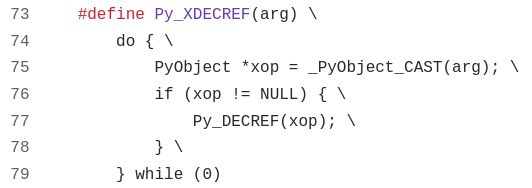
\includegraphics[width=0.7\textwidth, height=0.5\textheight]{docs/images/define}
\end{center}
\end{figure}
\end{itemize}
\end{frame}

\begin{frame}{یک سیستم پردازشگر زبان - \lr{Compiler}}
\begin{figure}[H]
\begin{center}
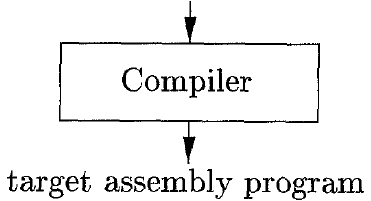
\includegraphics[width=0.5\textwidth, height=0.5\textheight, angle=0.6]{docs/images/compiler}
\end{center}
\end{figure}
\end{frame}

\begin{frame}{یک سیستم پردازشگر زبان - \lr{Assembler}}
\begin{figure}[H]
\begin{center}
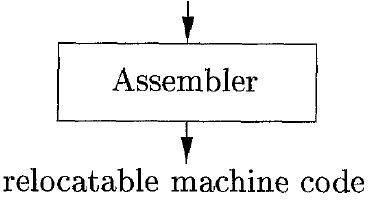
\includegraphics[width=0.5\textwidth, height=0.5\textheight, angle=0.6]{docs/images/assembler}
\end{center}
\end{figure}
\end{frame}

\begin{frame}{یک سیستم پردازشگر زبان - \lr{Linker/Loader}}
\begin{figure}[H]
\begin{center}
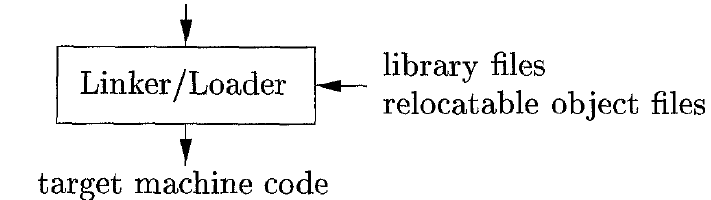
\includegraphics[width=0.75\textwidth, height=0.5\textheight, angle=0.4]{docs/images/linkerloader}
\end{center}
\end{figure}
\end{frame}
\section{ساختار یک کامپایلر}
\begin{frame}{ساختار کلی}
\begin{itemize}\itemr
\item[-]
تا کنون به کامپایلر به عنوان یک جعبه دارای ورودی خروجی نگاه می‌کردیم،
\item[-]
اما اگر این جعبه را باز کنیم، با دو قسمت اصلی در کامپایلر‌ها مواجه می‌شویم:
\begin{enumerate}\itemr
\item 
آنالیز
\item 
سنتز
\end{enumerate}
\end{itemize}
\end{frame}

\begin{frame}{آنالیز}
\begin{itemize}\itemr
\item[-]
این قسمت، \lr{source code} را به قسمت‌های مختلفی می‌شکند،

\item[-]
و قواعد گرامی را به قسمت‌های مختلف تحمیل می‌کند.

\item[-]
این قسمت، اگر قسمتی را مخالف قوانین و گرامر زبان پیدا کند، پیام‌های مطلع کننده‌ای به کار نشان می‌دهد که ورودی را اصلاح کند.

\item[-]
و در پایان این قسمت، داده ساختاری به نام \lr{\textit{symbol table}} را تولید می‌کند که تقریبا در تمامی گام‌های کامپایل (که در ادامه به آنها پرداخته می‌شود،) استفاده می‌شود.
\end{itemize}
\end{frame}

\begin{frame}{سنتز}
\begin{itemize}\itemr
\item[-]
قسمت سنتز، بعد از رد شدن از تمامی مراحل قسمت آنالیز، خروجی مورد نیاز ما را تولید می‌کند.

\item[-]
به قسمت آنالیز 
\lr{front-end}
و قسمت سنتز
\lr{back-end}
هم گفته می‌شود.
\end{itemize}
\end{frame}

\begin{frame}{\lr{front-end}}
\begin{figure}[H]
\begin{center}
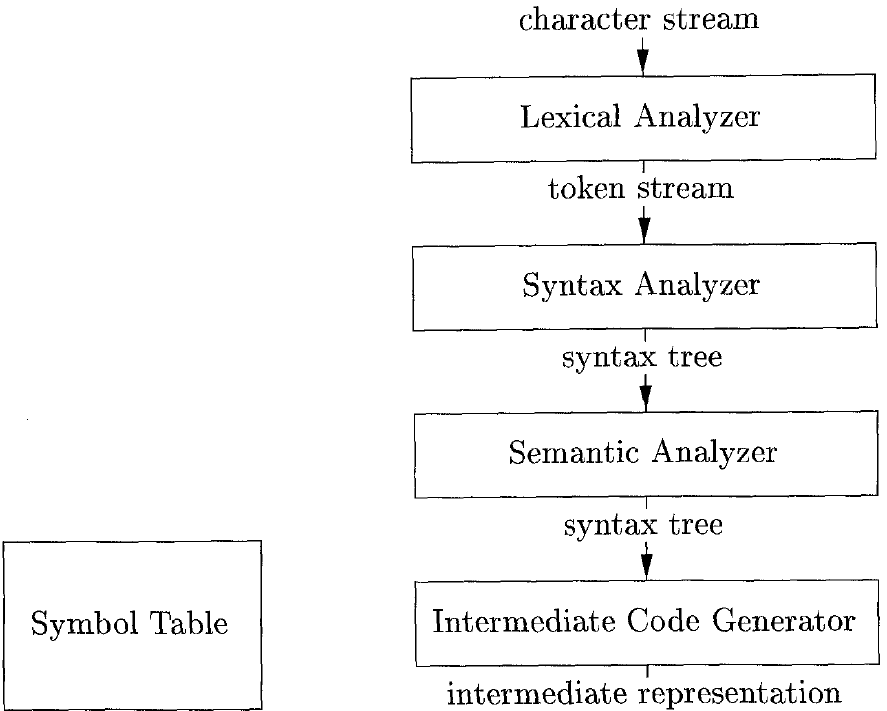
\includegraphics[width=0.5\textwidth, height=0.8\textheight, angle=-0.5]{docs/images/front}
\end{center}
\end{figure}
\end{frame}

\begin{frame}{\lr{back-end}}
\begin{figure}[H]
\begin{center}
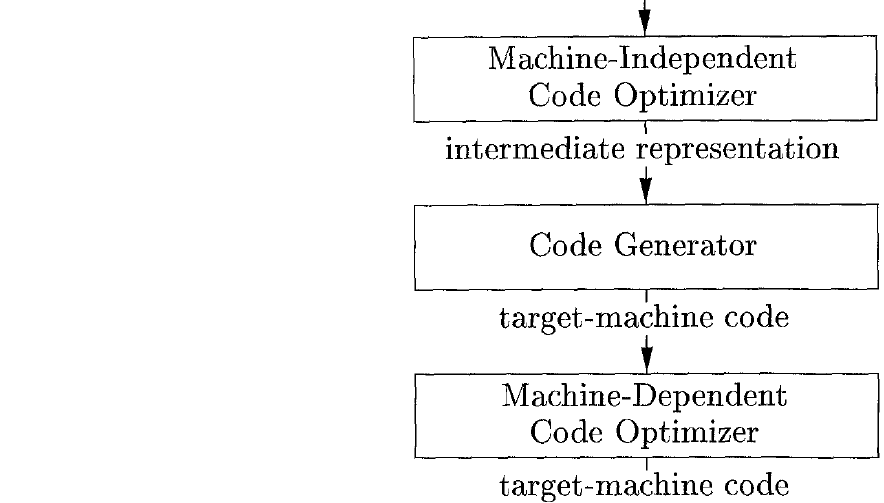
\includegraphics[width=0.5\textwidth, height=0.6\textheight, angle=-0.5]{docs/images/back}
\end{center}
\end{figure}
\end{frame}

\end{document}
